\documentclass{beamer}
\usepackage[russian]{babel}
\usetheme{metropolis}

\usepackage{amsthm, amssymb}
\setbeamertemplate{theorems}[numbered]

\setbeamercolor{block title}{use=structure,fg=white,bg=gray!75!black}
\setbeamercolor{block body}{use=structure,fg=black,bg=gray!20!white}

\usepackage[T2A]{fontenc}
\usepackage[utf8]{inputenc}

\usepackage{hyphenat}
\usepackage{amsmath}
\usepackage{graphicx}

\usepackage{booktabs}

\AtBeginEnvironment{proof}{\renewcommand{\qedsymbol}{}}{}{}

\title{
Микроэкономика-I
}
\author{
Павел Андреянов, PhD
}

\begin{document}

\maketitle

\section{Свойства полезности в $\mathbb{R}^n$}

\begin{frame}{Свойства полезности в $\mathbb{R}^n$}

Напомним, на чем мы остановились

\begin{definition}
Полезность $U$ \alert{непрерывна}, если ее $L_+$, $L_-$ - замкнутые.
\end{definition}

\begin{definition}
Полезность $U$ \alert{вогнута}, если ее подграфик - выпуклый.
\end{definition}

Забегая вперед, сегодня будет еще одно определение, но я помещу его тут, потому что они хорошо смотрятся вместе.

\begin{definition}
Полезность $U$ \alert{квази вогнута}, если ее $L_+$ - выпуклые.
\end{definition}

\end{frame}

\begin{frame}{Вогнутость}

Вернемся к \alert{вогнутости}.

К сожалению, не все могут быстро в уме нарисовать график или подграфик функции от двух переменных, а тем более от трех переменных, и сказать выглядит он как колпак или нет.

Например, $\sqrt{xy}$ или $x^2y^2$.

В таких случаях мы применяем \alert{критерий Сильвестра} (его покажу на следующем слайде) для подтверждения или отрицания вогнутости функции.

\end{frame}

\section{Критерий Сильвестра}

\begin{frame}{Критерий Сильвестра}

\begin{columns}
\begin{column}{0.5\textwidth}
   \alert{Джеймс Джозеф Сильвестер} (James Joseph Sylvester) английский и американский математик второй половины 19 века, профессор Университета Джон Хопкинс и позже Оксфорда. Изобрел матрицы, дискриминанты, и, собственно, критерий имени самого себя. \\ Этот критерий заключается в проверке отрицательной определенности матрицы Гесса.
\end{column}
\begin{column}{0.5\textwidth}  %%<--- here
    \begin{center}
     \includegraphics[width=1\textwidth]{sylvester.jpeg}
     \end{center}
\end{column}
\end{columns}

\end{frame}

\begin{frame}{Критерий Сильвестра}

Матрица Гесса $\nabla^2 U$, она же <<матрица вторых производных>> является симметричной а значит диагонализуемой.

Предположим, что в некотором базисе 

$$\nabla^2 U \sim \begin{pmatrix}
  \lambda_1 & 0 & 0 \\
  0 & \lambda_2 & 0 \\
  0 & 0 & \lambda_3
\end{pmatrix}$$

\end{frame}

\begin{frame}{Критерий Сильвестра}

Пусть собственные значения $\lambda_i$ все ненулевые.

Есть два важных случая

\begin{itemize}
  \item все знаки строго отрицательные - это \alert{строго вогнутая} функция, такая как $-x^2-y^2-z^2$
  \item все знаки строго положительные - это \alert{строго выпуклая} функция, такая как $x^2+y^2+z^2$
\end{itemize}

Любой другой вариант ненулевых знаков собственных значений это тоже не вогнутая функция.

\end{frame}

\begin{frame}{Критерий Сильвестра - I}

В диагональном случае, угловые миноры (которых 3 штуки для $n = 3$) строго вогнутой функции характеризуются

\begin{itemize}
  \item $\det M_{1} = \lambda_1 < 0$
  \item $\det M_{1,2} = \lambda_1 \cdot \lambda_2 > 0$
  \item $\det M_{1,2,3} = \lambda_1 \cdot \lambda_2 \cdot \lambda_3 < 0$
\end{itemize}

Проверка чередования знаков угловых миноров называется \alert{Критерием Сильвестра знаковой определенности матрицы}. Более того, он работает в любом базисе.

\end{frame}

\begin{frame}{Критерий Сильвестра - I}

А что если некоторые собственные значения равны нулю

Есть два важных случая

\begin{itemize}
  \item все знаки отрицательные или нулевые - это просто \alert{вогнутая} функция
  \item все знаки положительные или нулевые - это просто \alert{выпуклая} функция
\end{itemize}

Функция может быть (нестрого) выпуклой и вогнутой одновременно, например, линейная.

\end{frame}

\begin{frame}{Критерий Сильвестра - II}

В диагональном случае, главные миноры (которых 7 штук для $n = 3$) нестрого вогнутой функции характеризуются

\begin{itemize}
  \item $\det M_{1} = \lambda_1 \leqslant 0$
  \item $\det M_{2} = \lambda_2 \leqslant 0$
  \item $\det M_{3} = \lambda_3 \leqslant 0$
  \item $\det M_{1,2} = \lambda_1 \cdot \lambda_2 \geqslant 0$
  \item $\det M_{2,3} = \lambda_2 \cdot \lambda_3 \geqslant 0$
  \item $\det M_{1,3} = \lambda_1 \cdot \lambda_3 \geqslant 0$
  \item $\det M_{1,2,3} = \lambda_1 \cdot \lambda_2 \cdot \lambda_3 \leqslant 0$
\end{itemize}

Проверка чередования знаков главных миноров называется \alert{Критерием Сильвестра знаковой полу-определенности матрицы} и работает в любом базисе.

\end{frame}

\begin{frame}{Критерий Сильвестра - подытожим}

Первый критерий:
\begin{gather*} F \text{ стр. вогнутая } \Leftrightarrow v \nabla^2 F v < 0 \\
\Leftrightarrow \text{угловые миноры знакочередуются и }\neq 0\end{gather*}

Второй критерий:
\begin{gather*}F \text{ вогнутая } \Leftrightarrow v \nabla^2 F v \leqslant 0 \\ 
\Leftrightarrow \text{главные миноры знакочередуются}\end{gather*}

Второй критерий известен меньше, потому что главных миноров очень очень много и их проверка не всегда является практичной. 

Но для $n = 3$ можно сделать, главных миноров $7$.

\end{frame}


\section{А если он не работает?}

\begin{frame}{А если он не работает?}

Если не удается применить критерий, есть другие приемы.

\begin{itemize}
  \item линейные функции - вогнуты
  \item сумма вогнутых функций - вогнута
  \item минимум (любого числа) вогнутых функций - вогнут
  \item монотонно возрастающее преобразование вогнутой функции - вогнуто, если это преобразование само вогнуто. 
\end{itemize}

Например, такими преобразованиями являются $\sqrt{x}, \log(x)$ но не являются $\exp(x), x^2$.
 
\end{frame}

\begin{frame}{А если он не работает?}

Потренируемся в проверке вогнутости

\begin{itemize}
  \item $x y$
  \item $x^{1/3} y ^{2/3}$
  \item $x + 2y + 3 z$
  \item $x y + \min(x, y)$
  \item $\min(x y, z + x)$
  \item $\sqrt{x^{1/3} y ^{2/3} + z}$
\end{itemize}

Приведите пример не вогнутой фунцкии?
 
\end{frame}

\section{Проблемы с вогнутостью}

\begin{frame}{Вогнутость}

К сожалению, с вогнутостью есть проблема. 

Три полезности
\begin{itemize}
  \item $x^2y^2$
  \item $\sqrt{xy}$
  \item $\log x + \log y$
\end{itemize}
задают одни и те же предпочтения.

Однако, 2 из них вогнутые а одна - вовсе нет.

Попробуйте определить какие?

\end{frame}

\begin{frame}{Вогнутость}

Проблема в том, что монотонные преобразования легко ломают вогнутость, если они сами при этом не являются вогнутыми, достаточно накрутить несколько экспонент.

Поэтому экономисты придумали свою собственную почти-вогнутость, или \alert{квази вогнутость} (quasi- от лат. почти).

\end{frame}

\section{Квази вогнутость}

\begin{frame}{Квази вогнутость}

Проверка квази-вогнутости опирается на форму верхних Лебеговых множеств (вместо формы подграфика)...

\begin{definition}
Полезность $U$ \alert{вогнута}, если ее подграфик - выпуклый. 
\end{definition}

\begin{definition}
Полезность $U$ \alert{квази вогнута}, если все ее $L_{+}(x)$ - выпуклы. 
\end{definition}

...а следовательно инвариантна к монотонно возрастающим преобразованиям.

\end{frame}

\begin{frame}{Квазивогнутость}
\centering рисунок в $\mathbb{R}^n$
\begin{figure}[hbt]
\centering
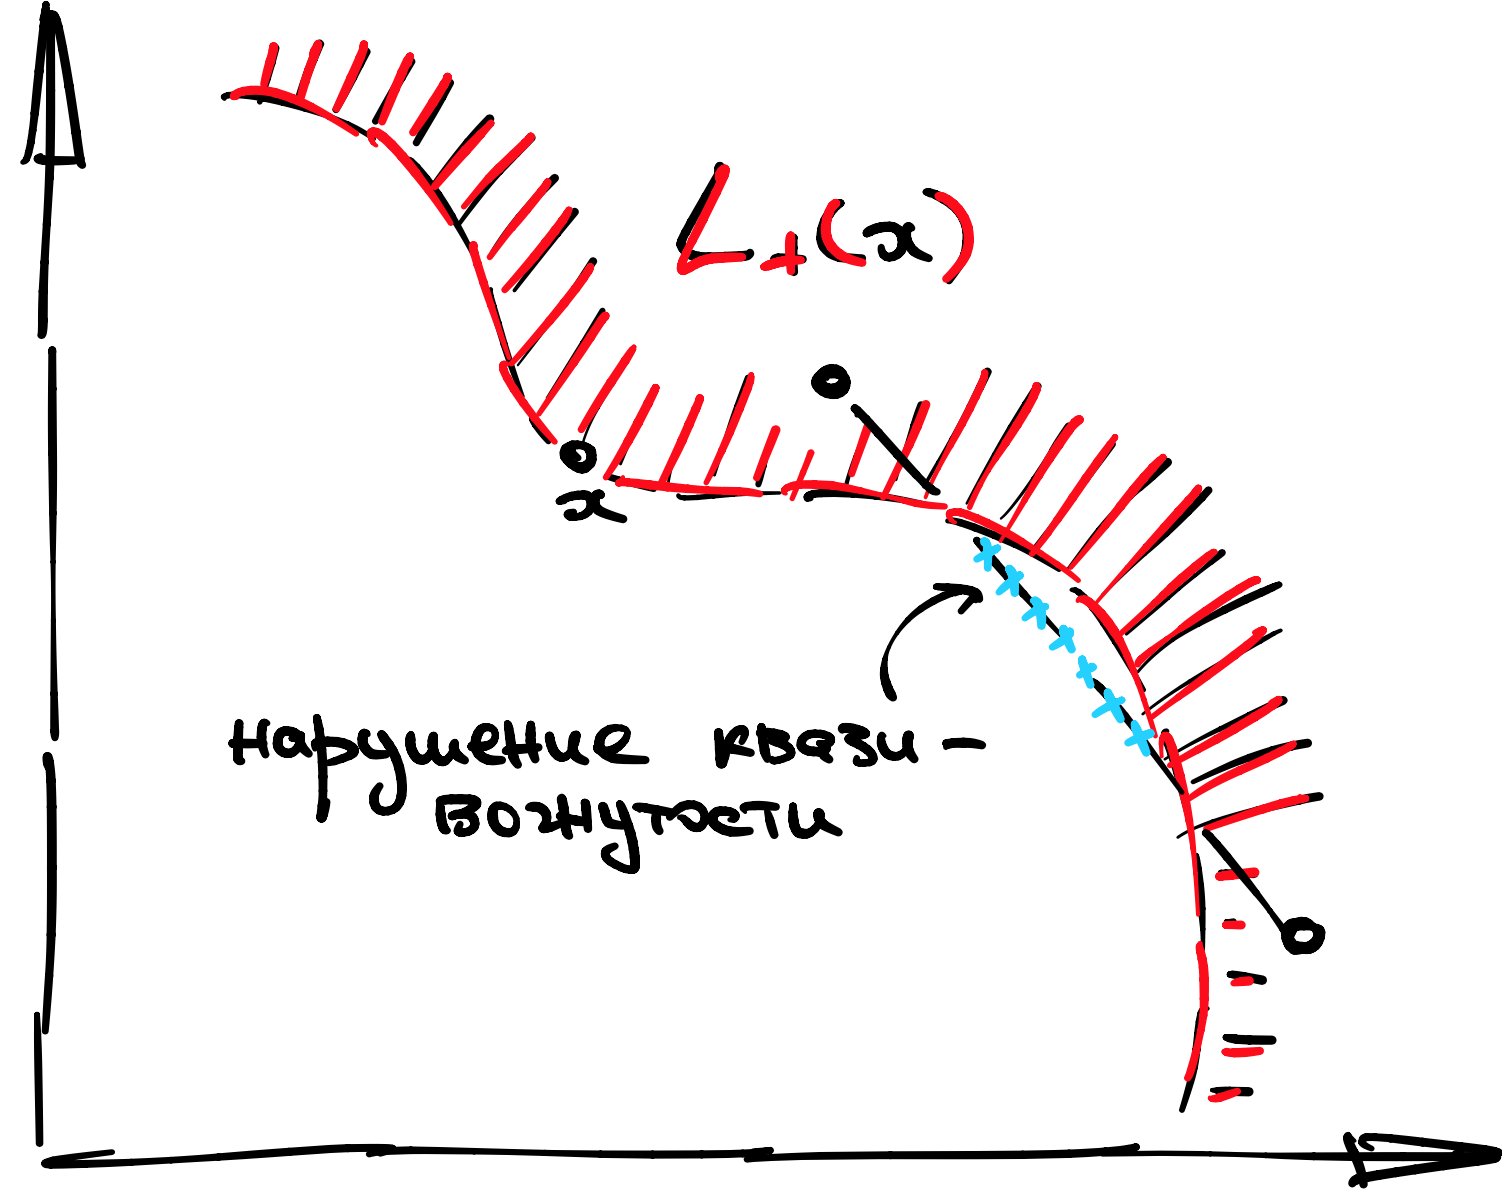
\includegraphics[width=.7 \textwidth]{not_quasi.png}
\end{figure}
\end{frame}

\begin{frame}{Квази вогнутость}

Любопытный факт

Посколько $L_+$ является как бы тенью (проекцией на $\mathbb{R}^n$) верхнего отреза подграфика (живущего в $\mathbb{R}^{n+1}$), то...

...\alert{из вогнутости автоматически следует квази вогнутость}.

\end{frame}

\begin{frame}{Квази вогнутость}

Есть также эквивалентное определение квази вогнутости

\begin{definition}
Полезность $U$ \alert{квази вогнута} в $X$, если для любых $x, y \in X$:
$$ \forall \alpha \in (0,1): U(\alpha x + (1-\alpha) y)) \geqslant \min(U(x), U(y))$$
\end{definition}
в стиле примерно такого же определения вогнутости
\begin{definition}
Полезность $U$ \alert{вогнута}, если для любых $x, y \in X$: 
$$ \forall \alpha \in (0,1): U(\alpha x + (1-\alpha) y)) \geqslant \alpha U(x) + (1-\alpha) U(y)$$
\end{definition}

\end{frame}

\begin{frame}{Квази вогнутость}
Любители алгебры могут убедиться, что \alert{из вогнутости действительно следует квази вогнутость} (но не наоборот).
\begin{proof}
\begin{align*} 
(1) : & \quad U(\alpha x + (1-\alpha) y)) \geqslant \alpha U(x) + (1-\alpha) U(y) \\
(2) : & \quad \alpha U(x) + (1-\alpha) U(y) \geqslant \min (U(x), U(y))\\
(1), (2) \quad \Rightarrow & \quad U(\alpha x + (1-\alpha) y)) \geqslant \min (U(x), U(y))
\end{align*}
\end{proof}

\end{frame}

\section{Зачем эта приставка квази-?}

\begin{frame}{Зачем эта приставка квази-?}

Чтобы ответить на этот вопрос, нужно сначала понять \alert{зачем нам нужна была вогнутость}? 

Короткий ответ - \alert{для единственности решения оптимизационных} задач с бюджетными (в общем случае выпуклыми) ограничениями.

Однако, \alert{квази вогнутость так же приводит к единственности} решений, при этом являясь менее требовательным к полезности - \alert{общую идею нарисую на доске}.

\end{frame}

\begin{frame}{Зачем эта приставка квази-?}

А если результат тот же - зачем платить больше? 

Действительно, если квази вогнутость однозначно слабее чем вогнутость, экономисту проще поверить в то что первая может быть выполнена в реальности.

При этом, повторюсь, \alert{как вогнутость так и квази вогнутость приводят к единственности решений в выпуклых задачах} (строгое определение выпуклой задачи дам чуть позже).
\end{frame}

\begin{frame}{Зачем эта приставка квази-?}

На самом деле, структура которую вогнутость налагает на полезность говорит не только о единственности решений, но также об отношении агента к риску, он его не любит. Это для нас сейчас - совершенно лишнее знание.

Квази вогнутость это та часть вогнутости, которая отвечает за единственность решений. 

Но кроме принципа Оккама \alert{есть и другие соображения в пользу квази вогнутости}.

\end{frame}


\begin{frame}{Неоднозначность полезности}

Напомню, что для любого строго монотонного преобразования $\varphi$, две полезности - $U(x)$ и $\varphi(U(x))$ - производят идентичное поведение у потребителей.  

Все ниже перечисленные полезности эквивалентны с точки зрения поведения потребителей
\begin{align*}
& x^2y^3,\\
& 2\log x + 3\log y,\\
& 2\log x + 3\log y + 1,\\
& 2(2\log x + 3\log y) + 1.
\end{align*}

\end{frame}

\begin{frame}{Неоднозначность вогнутости}

Напомню. что \alert{вогнутость} (часто) \alert{ломается при монотонных преобразованиях} полезности. 

В отличие от нее, \alert{квази вогнутость сохраняется при монотонных преобразованиях} полезности. 

Когда какое то свойство инвариантно к спецификации (или трансформации) полезности, экономисты такое очень любят.
\end{frame}

\begin{frame}{Неоднозначность вогнутости}

Итак, супер важный факт:

\begin{lemma}
Если $U(x)$ вогнута или квази вогнута, то $\varphi(U(x))$ квази вогнута для любой строго монотонно возраст-ей функции $\varphi$. 
\end{lemma}

Конечно, может так случиться, что $\varphi(U(x))$ все таки вогнута, это ничему не противоречит поскольку из вогнутости следует и квази вогнутость. Функция может быть вогнутой и квази вогнутой одновременно.
\end{frame}

\begin{frame}{Неоднозначность вогнутости}

Чтобы придумать алгебраичное доказательство, достаточно знать следующие свойства строго монотонно возрастающих функций $\varphi$:
 \begin{align*}
U(x) \leqslant U(y) \quad \Leftrightarrow \quad \varphi(U(x)) \leqslant \varphi(U(y))\\
U(x) \geqslant U(y) \quad \Leftrightarrow \quad \varphi(U(x)) \geqslant \varphi(U(y))\\
\min(\varphi(U(x)), \varphi(U(y))) = \varphi(\min(U(x),U(y)))
\end{align*}

\end{frame}

\section{Какие функции квази вогнуты?}

\begin{frame}{Какие функции квази вогнуты?}

Приведу несколько примеров

\begin{itemize}
  \item линейные
  \item вогнутые
  \item монотонно возрастающие преобразования вогнутых
  \item монотонные в $\mathbb{R}^1$
  \item однопиковые в $\mathbb{R}^1$
\end{itemize}

Продвинутое упражнение: приведите (нарисуйте) две функции (поверхности) в $\mathbb{R}^2$: монотонную и однопиковую; которые не являются квазивогнутыми.
\end{frame}

\section{Предпочтения}

\begin{frame}{Предпочтения}

Модель предпочтений более абстрактна чем полезность

\begin{itemize}
\item снова один агент
\item товары разделены на $n$ категорий
\item портфель (потр. корзина) это точка в $\mathbb{R}_{+}^{n}$	
\item категории, а также координаты обозначаются $x, y, z...$
\item множество доступных альтернатив $X \subset \mathbb{R}_{+}^{n}$
\end{itemize}

Однако вместо полезности $U: X \to \mathbb{R}$ у агента в голове зашито бинарное отношение $\succcurlyeq: X^2 \to \{0,1\}.$

\end{frame}

\begin{frame}{Предпочтения}

Напомню как визуализировать бинарное отношение на множестве альтернатив малой размерности, например 3.
$$
\begin{array}{c|ccc}
 \succcurlyeq & x & y & z\\
\hline
x & 1 & 1 & 0 \\
y & 0 & 1 & 1\\
z & 0 & 1 & 0
\end{array}
$$

$x \succcurlyeq y$ означает что $(x,y) \mapsto 1$.

$x \preccurlyeq y$ означает что $(y,x) \mapsto 1$.

Формально, бинарное отношение – это любое расположение ноликов и единичек внутри матрицы.

\end{frame}

\begin{frame}{Предпочтения}

Напомню, что для простоты вводятся дополнительные обозначения:

$x \sim y$ означает что $x \succcurlyeq y$ и $x \preccurlyeq y$.

$x \succ y$ означает что $x \succcurlyeq y$ но не $x \sim y$.

$x \prec y$ означает что $x \preccurlyeq y$ но не $x \sim y$.

Получаются пять интуитивных отношений сильного, слабого предпочтений и безразличия.

Однако какие попало матрицы писать не стоит.

\end{frame}

\begin{frame}{Предпочтения}

Поскольку у бинарного отношения есть экономическая интерпретация, это накладывает на него определенные ограничения, называемые \alert{аксиомами рациональности}.

\begin{definition}
Предпочтения $\succcurlyeq$	\alert{рациональны}, если
\begin{itemize}
\item для любыx $x, y \in X$, либо $x \succ y$ либо $y \succ x$ либо $y \sim x$.
\item для любой $x \in X$, всегда верно что $x \sim x$
\item для любыx $x, y, z \in X$: 
$$x \succcurlyeq y, y \succcurlyeq z \quad \Rightarrow \quad x \succcurlyeq z$$
\end{itemize}
\end{definition}
Последнее свойство - самое важное и называется \alert{транзитивностью}. 

\end{frame}

\begin{frame}{Предпочтения}

Рациональность накладывают структуру на то, как может заполняться матрица. 
$$ 
\begin{array}{c|ccc}
 \succcurlyeq & x & y & z\\
\hline
x & * & * & * \\
y & 0 & * & 1\\
z & 0 & 1 & *\\
\end{array}
$$
Попробуйте дозаполнить следующую матрицу так, чтобы предпочтения были рациональными.

\end{frame}

\section{Свойства предпочтений}

\begin{frame}{Предпочтения}
Переопределив естественным образом Лебеговы множества $L_{+}(x)$ и $L_{-}(x)$ в терминах предпочтений, мы автоматически получаем аналоги свойств предпочтений. Заодно, можно сразу дать определения монотонности и локальной ненасыщаемости для полезности и предпочтений.
\vspace*{-0.5cm}
\begin{table}
\begin{center}
\begin{tabular}{@{} |c|c|c| @{}}
 \hline
 предпочтения & полезности & определение \\ 
 \hline
 непрерывны & непрерывны & $L_+, L_-$ замкнуты \\ 
 \alert{выпуклы} & квази вогнуты & $L_+$ выпуклы \\ 
 - & вогнуты & подграфик выпуклый \\ 
 монотонны & монотонны & $L_{+}(x) + v \subset L_+(x), \ \forall v \in \mathbb{R}^n_+$\\
лок. ненас. & лок. ненас. & $\forall x,\varepsilon \ \exists y: |x-y|<\varepsilon, y \in L_{++}(x)$\\
 \hline
\end{tabular}
\end{center}
\end{table}

Тут, к сожалению, есть врожденный баг терминологии.
\end{frame}

\begin{frame}{Предпочтения}

Парадокс в том, что вогнутые (concave) полезности - квазивогнутые, однако, ассоциированы с выпуклыми предпочтениями. А выпуклые (convex) полезности, например $\max(x,y)$, с выпуклыми предпочтениями как раз никак не связаны и даже противоречат им. 

\end{frame}

\begin{frame}{Предпочтения}

Это происходит из того, что выпуклость - очень древнее слово в физике и те кто придумали выпуклые предпочтения (они были скорее всего физико-математиками) не задумались о том, что это приведет к конфликту в будущем.

Дело в том, что в физике все минимизируется (например, энергия), поэтому функции там выпуклые, а в экономике, наоборот, полезность максимизируется поэтому она вогнутая.

\end{frame}

\section{Прямая связь}

\begin{frame}{Прямая связь}

Предположим, что у вас уже есть откалиброванная полезность. Как вывести из нее модель предпочтений?

\begin{definition}
Будем говорить, что $U$ \alert{представляет} $\succcurlyeq$, если
$$ U(x) \geqslant U(y) \quad \Leftrightarrow \quad  x \succcurlyeq y.$$
\end{definition}

Должно быть понятно, что если предпочтения представлены $U$, то они будут обязательно рациональны, поскольку аксиомы рациональности копируются со свойств вещественных чисел. 

Также, любое свойство предпочтений, будь то непрерывность, монотонность или квази вогнутость, копируются на полезность которая его представляет.

\end{frame}

\section{Обратная связь}

\begin{frame}{Обратная связь}

Предположим, что у вас уже есть откалиброванные рациональные предпочтения в $X \subset \mathbb{R}^n$. Можно ли восстановить по ним хотя бы одну непротиворечивую полезность? 

Оказывается, что в простых случаях, действительно, можно.

\begin{lemma}
Если $X$ конечно, то для любых рациональных предпочтений $\succcurlyeq$ существует полезность $U$, представляющая $\succcurlyeq$.
\end{lemma}

Это легко доказать алгоритмически. Доказательство также легко переносится на случай счетного $X$.

В случае когда пространство альтернатив достаточно мощное, нам понадобится непрерывность предпочтений.

\end{frame}

\begin{frame}{Обратная связь}

\begin{columns}
\begin{column}{0.5\textwidth}
   \alert{Жерар Дебрё} (Gérard Debreu) французский экономист и математик, профессор экономики университета Беркли, лауреат нобелевской премии 1983 года по экономике. Работал над \alert{представлениями предпочтений потребителя при помощи вещественнозначных функций} и существованием равновесий в конкурентных рынках.
\end{column}
\begin{column}{0.5\textwidth}  %%<--- here
    \begin{center}
     \includegraphics[width=1\textwidth]{debreu.jpg}
     \end{center}
\end{column}
\end{columns}

\end{frame}

\begin{frame}{Обратная связь}

\begin{theorem}[Дебрё]
Если верно * то для любых \alert{рациональных и непрерывных предпочтений} $\succcurlyeq$ существует \alert{непрерывная полезность} $U$, представляющая $\succcurlyeq$.
\end{theorem}

Звездочка * это паравоз из условий, который меняется в зависимости от стиля доказательства. Есть несколько вариантов доказательства, из которых я вкратце расскажу два.

Сразу замечу, что отдельно проверять непрерывность $U$ не надо, так как она автоматически наследуется от $\succcurlyeq$.

\end{frame}

\begin{frame}{Обратная связь}
Первый вариант паровоза *: $X$ это выпуклое замкнутое подмножество $\mathbb{R}^n$, а еще $\succcurlyeq$ строго монотонный.

\begin{itemize}
  \item Шаг 1. Ищем экстремумы $\succcurlyeq$ и соединяем их хордой $Y$.
  \item Шаг 2. Элементарно строим полезность на $Y$.
  \item Шаг 3. Продолжаем полезность с $Y$ на весь $X$.
\end{itemize}

Последний, самый сложный, шаг звучит примерно так. 

Для любой точки $x$ вне $Y$ строим $L_{++}(x)$ который содержит верхний и $L_{--}(x)$ который содержит нижний конец хорды. Они не пересекаются, значит есть точка $y$ на хорде такая что $x \sim y$, следовательно, можно присвоить значение $U(x) := U(y)$. 

\end{frame}

\begin{frame}{Обратная связь}
Второй вариант паровоза *: $X$ сепарабельно и связно.

\begin{itemize}
  \item Шаг 1. Берем счетное, всюду плотное подмножество $Y$. В частности, если $X \subset \mathbb{R}^n$, можно взять, $Y :=\mathbb{Q} \cap X$.
  \item Шаг 2. Элементарно строим полезность на $Y$.
  \item Шаг 3. Продолжаем полезность с $Y$ на весь $X$.
\end{itemize}

Последний, самый сложный, шаг звучит примерно так. 

Для любой точки $x$ вне $Y$ строим $L_{++}(x)$ и $L_{--}(x)$. Если есть точка $y \in Y$ такая что $x \sim y$, можно присвоить значение $U(x) := U(y)$. В противном случае, полагаем
$$ U(x):= \dfrac{\sup_{y \in Y \cap L_{--}(x)} U(y) + \inf_{y \in Y \cap L_{++}(x)} U(y)}{2}.$$

\end{frame}


\section{Выбор}

\begin{frame}{Выбор}

Модель выбора максимально абстрактна

\begin{itemize}
\item снова один агент
\item товары разделены на $n$ категорий
\item портфель (потр. корзина) это точка в $\mathbb{R}_{+}^{n}$	
\item категории, а также координаты обозначаются $x, y, z...$
\item множество доступных альтернатив $X \subset \mathbb{R}_{+}^{n}$
\end{itemize}

Вместо полезности $U: X \to \mathbb{R}$...

или бинарного предпочтения $\succcurlyeq: X^2 \to \{0,1\}$...

у агента в голове зашито \alert{отображение выбора} $C: 2^X \to 2^X$. 

Что это значит?

\end{frame}

\begin{frame}{Выбор}

Это значит, что агент отображает подмножества в подмножества. Так же как и с предпочтениями, есть несколько естественных технических ограничений:

\begin{itemize}
  \item $C(Z) \neq \emptyset$
  \item $C(Z) \subset Z$
\end{itemize}

Для любого непустого меню $Z \subset X$. 

Есть еще третья, самая важная аксиома.

\end{frame}

\begin{frame}{Выбор}

Рассмотрим любые два портфеля $x, y \in X$ и два меню $Z,Z' \subset X$, таких что $x,y$ содержатся в обоих меню.

\begin{definition} 
\alert{Слабая аксиома выявленных предпочтений} (WARP): 

Если в первом меню $y$ был выбран (в присутствие $x$) то невозможно чтобы во втором меню $x$ был выбран (в присутствие $y$) но сам $y$ выбран не был.
\end{definition}

Интуитивно, выбирая $x$ но не $y$ во втором меню вы, по сути, озвучиваете что-то вроде строгого предпочтения $x$ над $y$. 

Тогда, в первом меню было бы странно выбрать $y$ в присутствие лучшего $x$.

\end{frame}

\begin{frame}{Выбор}

\begin{definition}
Будем говорить, что $C$ \alert{выявляет} (\alert{reveals}) $\succcurlyeq$, если
$$ x \succcurlyeq y \quad \Leftrightarrow \quad x \ \text{выбран в присутствие} \ y$$
\end{definition}
Отсюда моментально следует, что $x \succ y$ тогда и только тогда, когда $x$ выбран в присутствие $y$ но сам $y$ выбран не был в том же меню, как в условии WARP. 

Предполагая нарушение следствия WARP, во втором меню $y$ был выбран в присутствие $x$, что значит
$y \succcurlyeq x$, но это противоречит $x \succ y$.
\end{frame}

\begin{frame}{Выбор}
Таким образом, WARP является необходимым условием для рациональности выявленных предпочтений (\alert{revealed preference}). 

Более того, из рациональности выявленных предпочтений также следует (а значит является необходимым условием) так называемая сильная аксиома выявленных предпочтений, которая рассматривает последовательность из $n+1$ меню.

\end{frame}

\begin{frame}{Выбор}

\begin{definition} 
\alert{Сильная аксиома выявленных предпочтений} (SARP): 

Если $x_{i}$ был выбран в присутствии $x_{i-1}$, для $i = 1, ..., n$, то невозможно, чтобы в последнем меню $x_0$ был выбран (в присутствие $x_n$) но сам $x_n$ выбран не был.
\end{definition}

По сути, WARP это полнота, а SARP это еще и транзитивность выявленных предпочтений. Легко видеть, что из SARP следует WARP, то есть, сильная аксиома <<сильнее>> чем слабая.

\end{frame}

\begin{frame}{Выбор}

Обращаю внимание, что для условий/аксиом <<сильнее>> это <<хуже>>, потому что меньше надежды на то что оно выполнено. 

Мы всегда говорим <<сильное условие>> с сожалением.

Для теорем все наоборот, <<сильнее>> это <<лучше>>.

Более <<сильная>> теорема/доказательство это та у которой более <<слабые>> условия при тех же выводах, либо более <<сильные>> выводы при тех же условиях.

Мы говорим <<сильное доказательство>> с гордостью.

\end{frame}


\begin{frame}{Выбор}

Есть еще третья, обобщенная аксиома выявленных предпочтений (GARP), которая сильнее чем SARP и WARP. 

Они все звучат очень похоже и у них похожие условия, так что легко ошибиться. Мне кажется, в некоторых учебниках даже я видел неправильные определения.

Будьте аккуратны.

\end{frame}

\section{Заключение}

\begin{frame}{Заключение}

Мы продемонстрировали, что из любой полезности можно вывести рациональные предпочтения, а из рациональных предпочтений выбор со слабой и сильной  аксиомами.

С другой стороны, из любых непрерывных и рациональных предпочтений можно вывести непрерывную полезность - это Теорема Дебре.

Аналог обратной связи для выбора называется \alert{Теорема Африата}, для которой нужен таки GARP. Это очень продвинутый материал, анализ которого не входит в мой курс. 

\end{frame}

\begin{frame}{Заключение}

\begin{figure}[hbt]
\centering
\includegraphics[width=1 \textwidth]{arch.png}
\end{figure}

\end{frame}

\begin{frame}{Заключение}

Какой из всего этого можно сделать вывод?

Все три модели, в каком то смысле эквивалентны. Поэтому можно смело использовать ту, которая вам кажется удобнее. 

Чаще всего (99\% случаев) это полезность, но иногда это и предпочтения, например в анализе алгоритма Гейла-Шепли, при помощи которого вас распределили по факультетам. 

С другой стороны, аксиомы выбора недавно <<вылезли>> в новейших комбинаторных аукционах, поэтому от теории выбора тоже есть некоторый толк.

\end{frame}

%\section{Конец первой части лекции}
%
%\begin{frame}{План на вторую часть лекции (1 час)}
%
%Далее мы сфокусируемся только на полезностях и как оптимизировать их при различных ограничениях.
%
%\begin{itemize}
%  \item Начала оптимизации
%  \item Условия первого и второго порядка
%  \item Выпуклость задачи
%  \item Краевые и внутренние решения
%  \item Линии уровня и геом. анализ
%\end{itemize}
%
%
%\end{frame}
%
%\section{Начала оптимизации}
%
%\begin{frame}{Начала оптимизации}
%
%Любая оптимизационная задача – это две вещи:
%
%\begin{itemize}
%  \item функция $U$ которую мы максимизируем
%  \item область определения $X$ по которым мы максимизируем
%\end{itemize}
%
%Ключевыми факторами тут являются непрерывность и (квази-) вогнутость целевой функции, а также компактность и выпуклость области определения.
%
%\end{frame}
%
%\section{Существование}
%
%\begin{frame}{Существование}
%
%Существование решения, как правило, мы можем легко гарантировать при помощи следующей теоремы
%
%\begin{theorem}[Вейерштрасса]
%
%Непрерывная функция на (непустом) компакте гарантированно достигает своего минимума и максимума.
%\end{theorem}
%
%Что такое \alert{непрерывность} вы уже знаете, а \alert{компакт} в $\mathbb{R}^n$ - это просто ограниченное и замкнутое множество. 
%
%В контексте одномерной оптимизации, отрезок $[a,b]$ - это компакт, а $(a,b]$, $[a,b)$, $(a,b)$, $[a,\infty)$,$(a,\infty)$ - нет. 
%
%В экономике вам будут попадаться, в основном компакты, поэтому вопрос о существовании как правило стоит не остро.
%
%\end{frame}
%
%\section{Дифференциальный анализ}
%
%\begin{frame}{Дифференциальный анализ}
%
%Предположим, что функция на компакте не только непрерывна но еще и дифференциируема сколько угодно раз, такая задача называется \alert{гладкой}. Тогда оптимум может быть
%
%\begin{itemize}
%  \item либо на границе $X$
%  \item либо во внутренней точке $X$
%\end{itemize}
%
%В последнем случае обязательно выполнены \alert{условия первого порядка} (УПП), это один из самых фундаментальных результатов дифференциального анализа.
%
%\end{frame}
%
%\begin{frame}{УПП}
%
%Например, если функция $U(x, y, z)$ от трех переменных, и вы убедили себя, что решение надо искать внутри, то
%$$\text{УПП (FOC)}: \quad  \nabla U = 0$$ 
%должны выполняться в оптимальной точке $(x^{\ast}, y^{\ast}, z^{\ast})$. 
%
%Значок $\nabla$ означает взятие градиента функции $$ \nabla U = \begin{pmatrix} \partial U/\partial x \\ \partial U/\partial y \\ \partial U/\partial z \end{pmatrix}$$
%в соответствующей точке.
%
%\end{frame}
%
%\begin{frame}{УПП на границе}
%
%Например, если функция $U(x, y, z)$, и вы убедили себя, что решение надо искать на границе $F(x,y,z) = 0$, то
%$$\text{УПП (FOC)}: \quad  \nabla \mathcal{L} = 0, $$ 
%где $\mathcal{L}(x,y,z|\lambda) = U(x, y, z) - \lambda F(x,y,z)$ это \alert{Лагранжиан}.
%
%Значок $\nabla$ означает взятие градиента Лагранжиана по всем переменным включая множители Лагранжа $$ \nabla \mathcal{L} = \begin{pmatrix} \partial \mathcal{L}/\partial x \\ \partial \mathcal{L}/\partial y \\ \partial \mathcal{L}/\partial z \\ \partial \mathcal{L}/\partial \lambda \end{pmatrix}$$
%в соответствующей точке.
%
%\end{frame}
%
%
%\begin{frame}{Критические точки}
%
%Как правило, количество точек, в которых выполнены УПП, с Лагранжианом или без,  конечно. Оптимум может также находиться на каком-то изломе или иной аномалии границы области определения.
%
%Все такие точки называются \alert{критическими}, их мало, и оптимум гарантированно лежит в одном из них. 
%
%\end{frame}
%
%\begin{frame}{Критические точки}
%
%\begin{figure}[hbt]
%\centering
%\includegraphics[width=.8 \textwidth]{extrema.png}
%\end{figure}
%
%\end{frame}
%
%\begin{frame}{Ручной перебор}
%
%Если у вас по любой причине остался один кандидат, то он и является оптимумом, поскольку существование нам гарантирует Теорема Вейерштрасса. 
%
%Если же кандидатов несколько, то надо сравнивать значения функции руками и выбирать все точки с наибольшим значением. 
%
%Тупой перебор Критические точки может привести к неожиданно быстрому решению задачи.
%
%\end{frame}
%
%\begin{frame}{Пример 1}
%
%Промаксимизируем функцию $f(x) = (x-1)^2$ на отрезке $[0,3]$.
%
%\begin{itemize}
%  \item Задача гладкая на компакте
%  \item Решим УПП, получим первую критическую точку $x = 1$
%  \item Две других критические точки это $x = 0$ и $x = 3$
%  \item Сравним значения: $$f(0) = 1, \ f(1) = 0, \ f(3) = 4.$$
%\end{itemize}
%
%Получается, что в этой задаче один единственный оптимум в точке $x = 3$, причем до условий второго порядка у нас даже руки не дошли.
%
%\end{frame}
%
%\begin{frame}{УВП}
%
%Число внутренних точек, прошедших УПП, можно дополнительно сузить за счет условий второго порядка.
%$$\text{УВП (SOC)}: \quad  \nabla^2 U \ ? \ 0$$
%Если Гессиан во внутренней точке отрицательно полу-определен $\nabla^2 U \leqslant 0$ (собственные значения $\leqslant 0$), то это \alert{локальный максимум} и этот кандидат проходит отбор.
%
%Если Гессиан положительно определен $\nabla^2 U > 0$ (собственные значения $>0$), то это строгий \alert{локальный минимум} и этот кандидат точно не проходит отбор.
%
%Есть еще третий случай, когда собственные значения Гессиана имеют противоположные знаки, это \alert{седло} и оно тоже не проходит отбор.
%
%\end{frame}
%
%\section{Выпуклость}
%
%\begin{frame}{Выпуклость}
%
%К счастью, в экономике зачастую удается показать, что поверх непрерывности функция полезности
%
%\begin{itemize}
%\item либо вогнутая
%\item либо она монотонное преобразование вогнутой
%\item либо она квазивогнутая
%\end{itemize}
%
%Если, вдобавок, область определения - выпуклое множество, то условия второго порядка можно не проверять. Такие задачи называются \alert{выпуклыми}.
%
%\end{frame}
%
%\begin{frame}{Пример 2}
%
%Промаксимизируем функцию $f(x) = -(x-1)^2$ на отрезке $[0,3]$.
%
%\begin{itemize}
%  \item Задача гладкая и выпуклая на компакте
%  \item Решим УПП, получим первую критическую точку $x = 1$
%  \item Убедимся что он находится внутри области
%\end{itemize}
%
%Все, этот экстремум и есть решение.
%
%\end{frame}
%
%\begin{frame}{Пример 3}
%
%Промаксимизируем функцию $f(x) = -(x+1)^2$ на отрезке $[0,3]$.
%
%\begin{itemize}
%  \item Задача гладкая и выпуклая на компакте
%  \item Решим УПП, получим первую критическую точку $x = -1$
%  \item Однако он не попадает в область, то есть, его нет
%  \item Две других критических точки это $x = 0$ и $x = 3$
%  \item Сравним значения: $$f(0) = 1, \ f(3) = -16.$$
%\end{itemize}
%
%Получается, что в этой задаче один единственный оптимум в точке $x = 0$.
%
%\end{frame}
%
%\begin{frame}{Выпуклость}
%
%Очень важно уметь, глядя на задачу, определять выпуклая она или нет, чтобы не тратить время на анализ второго порядка. 
%
%Общий алгоритм решения гладких и выпуклых задач на компакте очень простой:
%
%\begin{itemize}
%\item ищем первую критическую точку, как будто решение внутреннее
%\item если не попало в область определения - ищем на границе
%\item не забываем про изломы и иные аномалии области определения, потому что они, формально, являются кандидатами на решение
%\end{itemize}
%
%\alert{В выпуклых задачах условия второго порядка выполнены автоматически}, их проверка - пустая трата времени.
%
%\end{frame}
%
%\section{Геометрический анализ}
%
%\begin{frame}{Линии уровня}
%
%Наконец, линии уровня - это очень удобный инструмент для быстрого отлова и классификации кандидатов на решение оптимизационной задачи...
%
%\begin{definition}
%\alert{Линией уровня} полезности $U$, проходящей через точку $x$ называется множество всех точек $y \in X$ таких, что $U(y) = U(x)$.
%\end{definition}
%
%... особенно в двумерном случае.
%
%\end{frame}
%
%\begin{frame}{Кривые безразличия}
%
%\begin{definition}
%\alert{Кривой безразличия} предпочтений $\succcurlyeq$, проходящей через точку $x$ называется множество всех точек $y \in X$ таких, что $x \sim y$. Другими словами, это пересечение $L_+(x)$ и $L_-(x)$.
%\end{definition}
%
%Совершенно ясно, что в контексте представлений предпочтений полезностями, кривая безразличия и линия уровня - это одно и то же.
%
%\end{frame}
%
%\section{Локальная ненасыщаемость}
%
%\begin{frame}{Локальная ненасыщаемость}
%
%\begin{definition}
%Предпочтения $\succcurlyeq$ \alert{локально ненасыщаемы} в $X$, если для любой точки $x \in X$ найдется сколь угодно близкая к ней точка $x' \in X$, такая что $x' \succ x$.
%\end{definition}
%
%\begin{definition}
%Полезность $U$ \alert{локально ненасыщаема} в $X$, если для любой точки $x \in X$ найдется сколь угодно близкая к ней точка $x' \in X$, такая что $U(x') > U(x)$.
%\end{definition}
%
%Почти все полезности, которые будут вам встречаться, локально ненасыщаемы. Интуитивно это означает что кривые безразличия - тонкие линии. Если кривая безразличия толстая - это явное нарушение локальной ненасыщаемости.
%
%\end{frame}
%
%\section{Примеры полезностей}
%
%\begin{frame}{Линейная полезность}
%
%Рассмотрим полезность вида: $U(x, y) = ax + by$. Тогда линия уровня ищется следующим образом: 
%\begin{gather*}
%c = ax + by\\
%c-ax = by\\
%y = \frac{c-ax}{b}
%\end{gather*}
%Линия уровня - это прямая вида $y = \alpha x + \beta$.
%
%Эта полезность гладкая, вогнутая и локально ненасыщаемая.
%
%\end{frame}
%
%\begin{frame}{Гиперболическая полезность}
%
%Рассмотрим полезность вида: $U(x, y) = a \log x + \log y$. Тогда линия уровня ищется следующим образом: 
%\begin{gather*}
%c =  a \log x + \log y\\
%e^{c} = x^a y\\
%y =\frac{e^{c}}{x^a}
%\end{gather*}
%Линия уровня - это гипербола вида $y = x^\alpha \beta$.
%
%Эта полезность гладкая, вогнутая и локально ненасыщаемая.
%
%\end{frame}
%
%\begin{frame}{Полезность минимум}
%
%Рассмотрим полезность вида: $U(x, y) = \min(ax, by)$. Тогда линия уровня ищется следующим образом: 
%\begin{gather*}
%c = \min(ax, by)\\
%\frac{c}{b}= \min(\frac{a}{b}x, y), \quad \frac{c}{a}= \min(x, \frac{b}{a}y)\\
%y = \frac{c}{b} \mathbb{I}(ax > c), \quad x = \frac{c}{a} \mathbb{I}(by > c)
%\end{gather*}
%Линия уровня - это конкатенация горизонтальной и вертикальной линий, соединенных вдоль $ax = by$.
%
%Эта полезность НЕгладкая, но непрерывная, вогнутая и локально ненасыщаемая.
%
%\end{frame}
%
%\section{Метод пристального взгляда}
%
%\begin{frame}{Метод пристального взгляда}
%
%Очень часто, в задачах есть выпуклое ограничение типа неравенства, например, бюджетное ограничение. A полезность вогнутая или квазивогнутая.
%
%В таком случае, оптимум можно охарактеризовать как точку касания выпуклой области определения с одним из выпуклых верхних Лебеговых множеств. Однако, \alert{метод пристального взгляда работает только для локально ненасыщаемых предпочтений}. 
%
%В маломерных задачах, эта точка ищется визуально, а точные ее координаты либо угадываются из симметрии, либо из каких то других соображений.
%
%\end{frame}
%
%\begin{frame}{Метод пристального взгляда}
%
%\begin{figure}[hbt]
%\centering
%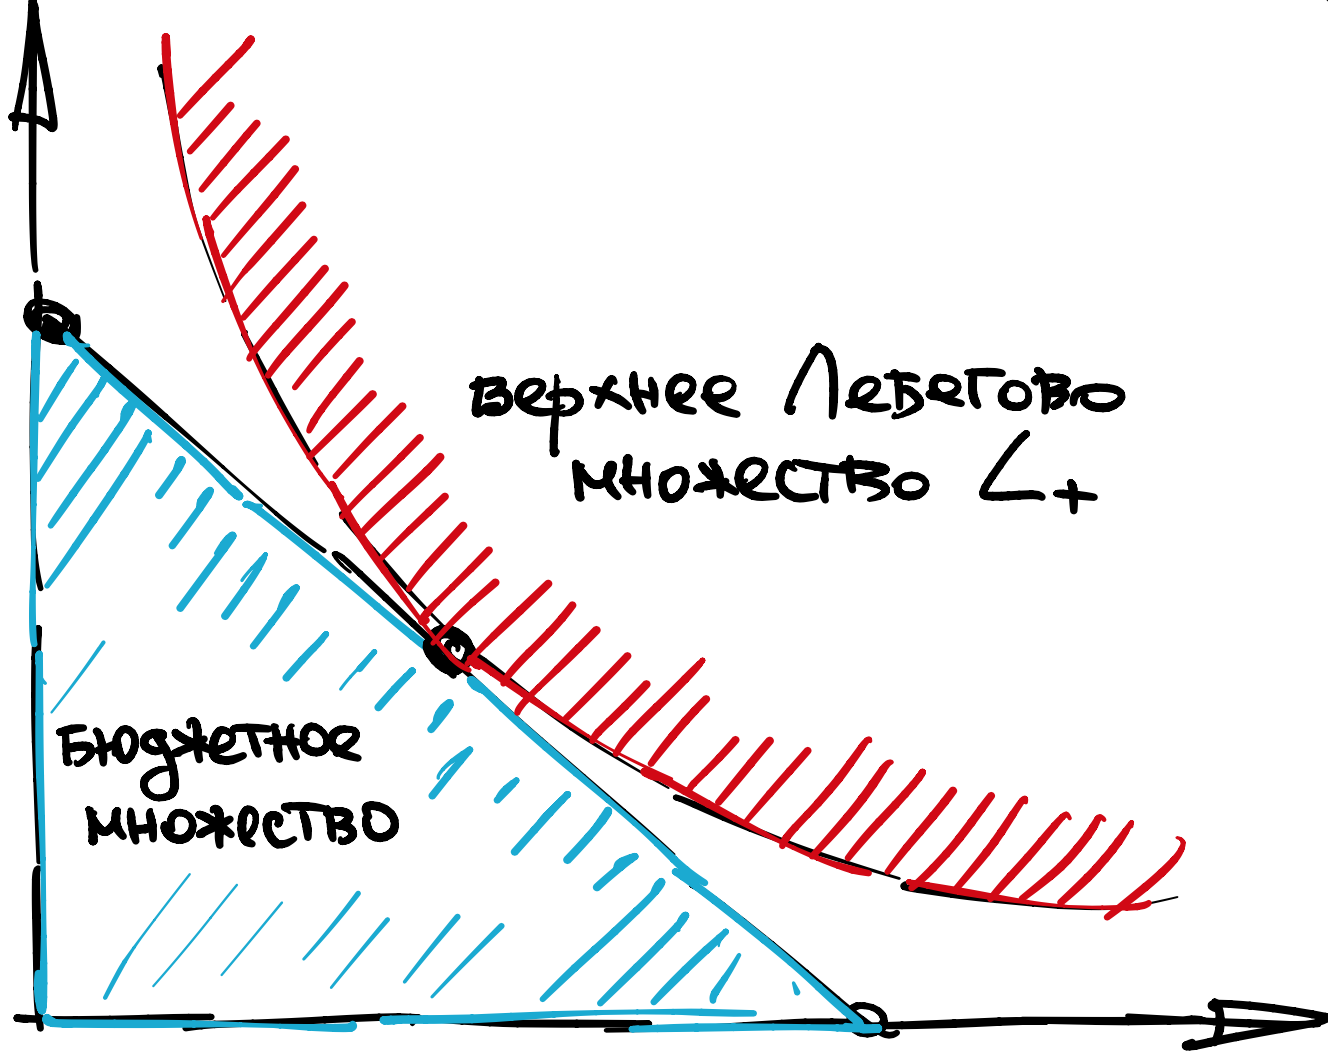
\includegraphics[width=.8 \textwidth]{tangency.png}
%\end{figure}
%
%\end{frame}
%\begin{frame}{Метод пристального взгляда}
%
%\begin{figure}[hbt]
%\centering
%\includegraphics[width=.8 \textwidth]{tang2.png}
%\end{figure}
%
%\end{frame}
%\begin{frame}{Метод пристального взгляда}
%
%\begin{figure}[hbt]
%\centering
%\includegraphics[width=.8 \textwidth]{tang3.png}
%\end{figure}
%
%\end{frame}
%
%\section{Конец второй части лекции}

\end{document}